\documentclass{ieeeojies}
\usepackage{cite}
\usepackage{amsmath,amssymb,amsfonts}
\usepackage{algorithmic}
\usepackage{graphicx}
\usepackage{textcomp}
\usepackage{array}
\usepackage[table]{xcolor}
\usepackage{multirow}
\usepackage{multicol}
\usepackage{float}

\def\BibTeX{{\rm B\kern-.05em{\sc i\kern-.025em b}\kern-.08em
    T\kern-.1667em\lower.7ex\hbox{E}\kern-.125emX}}

\begin{document}
\title{Investigating the Efficacy of Statistical, Machine Learning, and Deep Learning Approaches in Steel Stock Price Prediction}

\author{\uppercase{Le Xuan Quynh}\authorrefmark{1},
\uppercase{Nguyen Thi Thuy Hang\authorrefmark{2}, and Truong Gia Man}\authorrefmark{3}}

\address[1]{Faculty of Information Systems, University of Information Technology, (e-mail: 21520430@gm.uit.edu.vn)}
\address[2]{Faculty of Information Systems, University of Information Technology, (e-mail: 21520822@gm.uit.edu.vn)}
\address[3]{Faculty of Information Systems, University of Information Technology, (e-mail: 21521115@gm.uit.edu.vn)}

\markboth
{Author \headeretal: Le Xuan Quynh, Nguyen Thi Thuy Hang and Truong Gia Man}
{Author \headeretal: Le Xuan Quynh, Nguyen Thi Thuy Hang and Truong Gia Man}

\begin{abstract}
This study explores the prediction of stock prices for steel sector companies listed on the Ho Chi Minh Stock Exchange (HOSE). By employing a blend of statistical methods, machine learning techniques, and deep learning models, encompassing Vector Autoregressive Moving Average (VARMA), linear regression model, ARIMA, bagging models with decision trees and cost-sensitive, RNN, GRU, LSTM and Residual Networks (RESNET), our aim is to deliver precise forecasts of stock prices for Hoa Phat Group Joint Stock Company, Hoa Sen Group Joint Stock Company, and Nam Kim Steel Joint Stock Company. Through empirical analysis and comparative evaluation of these approaches, this study contributes to the advancement of stock price prediction methodologies within the steel sector.
\end{abstract}

\begin{keywords}
forecasting, steel sector, stock prices, statistics, machine learning, deep learning, VARMA, Bagging-RNN, ResNet, linear regression, ARIMA, RNN, GRU, LSTM
\end{keywords}

\titlepgskip=-15pt

\maketitle

\section{Introduction}
\label{sec:introduction}

Stock price forecasting remains a challenging yet crucial task for investors and financial analysts. Accurate predictions can provide valuable insights into potential investment opportunities and risks, thereby aiding in informed decision-making. This study aims to uncover patterns and trends that can enhance our understanding of future stock price movements, ultimately contributing to better investment strategies.

Various predictive models were employed in this study to analyze stock price data. These models include Linear Regression, VARMA (Vector Autoregressive Moving Average), ARIMA (Autoregressive Integrated Moving Average), Bagging Models with decision trees and cost-sensitive approaches, as well as recurrent neural network architectures such as RNN, GRU, LSTM, and ResNet. The dataset utilized in this research comprises five years of historical stock trading data from different Steel industry sectors.

The input data covers a period of five years, spanning from March 1, 2019, to March 1, 2024. The study's primary output focuses on predicting stock prices for the next 30, 60, and 90 days starting from March 1, 2024.

\section{Related Works}

In the article \cite{b1} focusing on Indonesia's export of oil and coal between 2002 and 2017, researchers employed the VARMA model to forecast production and quantity. Despite the initial non-stationarity of the dataset, confirmed by ACF and PACF analyses, they ensured data stationarity using the Augmented Dickey-Fuller unit root tests. Model selection was based on various information criteria, including AICC, HQC, AIC, and SBC. To enhance model accuracy, non-significant parameters such as those in AR-212, AR-221, and MA-121 were restricted. Furthermore, Granger causality tests indicated that oil exports were influenced solely by their own dynamics, not by coal exports.

The article \cite{b2} highlights the effectiveness of feature selection, decision tree models, bagging with decision trees, and cost-sensitive analysis in classifying diabetes patients using data from Sawanpracharak Regional Hospital in Thailand. It demonstrates a rational combination of methods to improve accuracy in classification applied to an important medical issue like diabetes patient classification. The article illustrates that feature selection and data processing require carefulness and a deep understanding of the specific problem. Improvement from feature selection is only a small part of the research process; applying cost-sensitive analysis methods can provide crucial information for medical decisions aligned with the initial goal of analyzing and predicting stock prices: providing insights into applying data analysis methods to complex financial issues.\\

In the study \cite{b3} conducted by a group of students from Sogang University in Seoul, short-term load forecasting based on ResNet and LSTM was investigated. The research began by utilizing the ResNet model for load forecasting and then proposed a novel method for Short-Term Load Forecasting (STLF) by exploiting a combined ResNet/LSTM model. The strength of ResNet lies in image recognition, with the study focusing on detecting graphs within the data to produce results.

\section{Materials}
\subsection{Dataset}
The primary objective of this research revolves around forecasting stock price movements within the steel sector. To achieve this goal, we utilize three distinct datasets sourced from reputable financial data providers. Specifically, the stock price data for Hoa Phat Group Joint Stock Company (HPG), Hoa Sen Group Joint Stock Company (HSG), and Nam Kim Steel Joint Stock Company (NKG) were collected from established stock market platforms. These datasets cover the period from March 1, 2019, to March 1, 2024, and encompass essential features pertinent to stock market analysis and prediction.


\subsection{Descriptive Statistics}
\begin{table}[H]
  \centering
  \caption{HPG, HSG, NKG’s Descriptive Statistics}
\begin{tabular}{|>{\columncolor{red!20}}c|c|c|c|}
    \hline
     \rowcolor{red!20} & HPG & HSG & NKG \\ \hline
     Count & 1252 & 1252 & 1252 \\ \hline
     Mean & 22,135 & 16,657 & 15,568\\ \hline
   %  Std & 10,778 & 6,359 & 22,722\\ \hline
     Min & 7,412 & 3,283 & 2,891\\ \hline
   %  25\% & 18,971 & 9,040 & 38,932\\ \hline
    % 50\% & 30,645 & 11,242 & 62,970\\ \hline
     %75\% & 35,893 & 18,400 & 77,008\\ \hline
     Max & 43,896 & 41,542 & 44,966\\ \hline
\end{tabular}
\end{table}

\begin{figure}[H]
    \centering
    \begin{minipage}{0.23\textwidth}
    \centering
    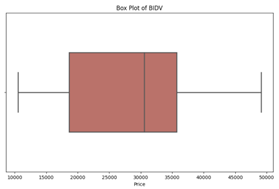
\includegraphics[width=1\textwidth]{bibliography/Figure/BIDVboxplot.png}
    \caption{BIDV stock price's boxplot}
    \label{fig:1}
    \end{minipage}
    \hfill
    \begin{minipage}{0.23\textwidth}
    \centering
    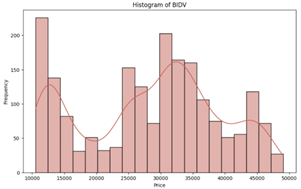
\includegraphics[width=1\textwidth]{bibliography/Figure/BIDVhist.png}
    \caption{BIDV stock price's histogram}
    \label{fig:2}
    \end{minipage}
\end{figure}

\begin{figure}[H]
    \centering
    \begin{minipage}{0.23\textwidth}
    \centering
    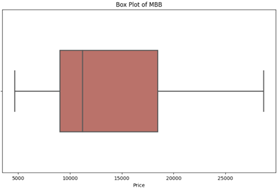
\includegraphics[width=1\textwidth]{bibliography/Figure/MBboxplot.png}
    \caption{MBB stock price's boxplot}
    \label{fig:1}
    \end{minipage}
    \hfill
    \begin{minipage}{0.23\textwidth}
    \centering
    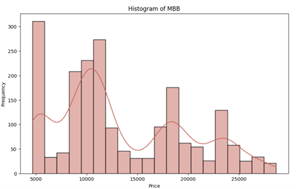
\includegraphics[width=1\textwidth]{bibliography/Figure/MBBhist.png}
    \caption{MBB stock price's histogram}
    \label{fig:2}
    \end{minipage}
\end{figure}

\begin{figure}[H]
    \centering
    \begin{minipage}{0.23\textwidth}
    \centering
    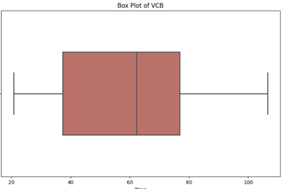
\includegraphics[width=1\textwidth]{bibliography/Figure/VCBboxplot.png}
    \caption{VCB stock price's boxplot}
    \label{fig:1}
    \end{minipage}
    \hfill
    \begin{minipage}{0.23\textwidth}
    \centering
    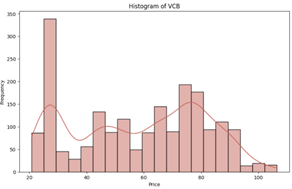
\includegraphics[width=1\textwidth]{bibliography/Figure/VCBhist.png}
    \caption{VCB stock price's histogram}
    \label{fig:2}
    \end{minipage}
\end{figure}

\section{Methodology}
\subsection{Linear Regression}
Regression analysis is a tool for building mathematical and statistical models that characterize relationships between a dependent variable and one or more independent, or explanatory, variables, all of which are numerical. This statistical technique is used to find an equation that best predicts the y variable as a linear function of the x variables.
A multiple linear regression model has the form: 
\[Y=\beta_0+\beta_1X_1+\beta_2X_2+\cdots+\beta_kX_k+\varepsilon\]
Where:\\
	\indent\textbullet\ Y is the dependent variable (Target Variable).\\
	\indent\textbullet\ \(X_1, X_2, \ldots, X_k\) are the independent (explanatory) variables.\\
	\indent\textbullet\ \(\beta_0\) is the intercept term.\\
	\indent\textbullet\ \(\beta_1,..., \beta_k\) are the regression coefficients for the independent variables.\\
	\indent\textbullet\ \(\varepsilon\) is the error term.
\subsection{ARIMA}
\subsection{VARMA}
VARMA modeling is a tool for building mathematical and statistical models that characterize relationships between multiple time series variables, all of which are numerical and evolve over time and producing linear forecasting. This statistical technique is used to find a set of equations that best predict a vector of variables as a function of their own past values and past shocks (unexpected events).VARMA model has the form:
\begin{equation}
\begin{split}
\mathbf{Y}_t &= \mathbf{\Phi}_1 \mathbf{Y}_{t-1} + \mathbf{\Phi}_2 \mathbf{Y}_{t-2} + \dots + \mathbf{\Phi}_p \mathbf{Y}_{t-p} \\
&\quad + \mathbf{\epsilon}_t + \mathbf{\Theta}_1 \mathbf{\epsilon}_{t-1} + \mathbf{\Theta}_2 \mathbf{\epsilon}_{t-2} + \dots + \mathbf{\Theta}_q \mathbf{\epsilon}_{t-q}
\end{split}
\end{equation}
\\
Where: \\ 
         \indent\textbullet\ \(\mathbf{Y}_t\)\ is a vector containing the values of the k variables at time t. \\
         \indent\textbullet\ \(\mathbf{\Phi}_1,\,\mathbf{\Phi}_2, \ldots, \mathbf{\Phi}_n\)\ are matrices of coefficients that capture the autoregressive (AR) relationships, showing how past values of the variables influence their current values. \\
         \indent\textbullet\ \textbf{p} is the order of the AR component (the number of past time steps included). \\
         \indent\textbullet\ \({\epsilon}(t)\) is  a vector of error terms (shocks or innovations) at time \textit{t}. \\
         \indent\textbullet\ \({\Theta}_1, {\Theta}_2, \ldots ,{\Theta}_q\) are matrices of coefficients that capture the moving average (MA) relationships, showing how past shocks influence the current values of the variables. \\
         \indent\textbullet\ \textbf{q} is the order of the MA components (the number of past shocks included). 
\subsection{Bagging-RNN}
\subsection{RNN}
Recurrent Neural Networks (RNNs) are deep learning models that can be utilized for time series analysis, with recurrent connections that allow them to retain information from previous time steps.The below equation represent a RNN cell:
\[h_t=tanh⁡(W_x x_t+W_h h_(t-1)+b) \]
Where: \\ 
         \indent\textbullet\ \(\mathbf x\)\ is the input of the current time step (present value). \\
         \indent\textbullet\ \(\mathbf h\)\ is the hidden state of the previous time step (past value). \\
         \indent\textbullet\ \(\mathbf b\)\ is bias. \\
         \indent\textbullet\ \(\mathbf W\)\ is The weights of the RNN are updated through a backpropagation in time (BPTT) algorithm. \\
\subsection{GRU}
\subsection{LSTM}

Long Short-Term Memory (LSTM) networks \cite{b4} have emerged as a prominent architecture in deep learning, particularly for tasks involving sequential data. LSTMs address the vanishing gradient problem \cite{b5} that plagues traditional Recurrent Neural Networks (RNNs), enabling them to effectively capture long-term dependencies.

The fundamental building block of an LSTM is the memory cell, which maintains its state over time. This cell \cite{b4} is equipped with three gates: the forget gate, input gate, and output gate. These gates regulate the flow of information into and out of the cell, allowing the LSTM to selectively retain or discard information. The forget gate determines which information from the previous state to forget, the input gate controls what new information to add to the cell state, and the output gate decides what information to output based on the cell state and current input.
\begin{align*}
  \text{Forget Gate:} \quad & f_t = \sigma(W_f [h_{t-1}, x_t] + b_f) \\
  \text{Input Gate:} \quad & i_t = \sigma(W_i [h_{t-1}, x_t] + b_i) \\
  & \tilde{C}_t = \tanh(W_C [h_{t-1}, x_t] + b_C) \\
  \text{Output Gate:} \quad & o_t = \sigma(W_o [h_{t-1}, x_t] + b_o) \\
  \text{Cell State:} \quad & C_t = f_t * C_{t-1} + i_t * \tilde{C}_t \\
  \text{Hidden State:} \quad & h_t = o_t * \tanh(C_t)
\end{align*} 
\\
Variables: \\
         \indent\textbullet\ \textbf{\(\mathbf{x}_t\)}: The input vector at time step (t). \\
         \indent\textbullet\ \textbf{\(\mathbf{h}_t\)}: The hidden state (output) at time step (t). \\
         \indent\textbullet\ \textbf{\(\mathbf{C}_t\)}: The cell state (internal memory) at time step (t). \\
         \indent\textbullet\ \textbf{\(\mathbf{W}_f,\, \mathbf{W}_i,\, \mathbf{W}_C,\ \mathbf{W}_o,\)}: Weight matrices for the forget, input, cell, and output gates, respectively. \\ 
         \indent\textbullet\ \textbf{\(\mathbf{b}_f,\, \mathbf{b}_i,\, \mathbf{b}_C,\ \mathbf{b}_o,\)}: Bias vectors for the forget, input, cell, and output gates, respectively. \\
\\
Functions: \\
         \indent\textbullet\ \(\sigma\): The sigmoid activation function, which squashes values between 0 and 1, representing how much information to let through the gate. \\ 
         \indent\textbullet\ \(\tanh\): The hyperbolic tangent activation function, which squashes value between -1 and 1, used to regulate the cell state. \\ 
\\
Interpretations: \\
         \indent\textbullet\ \textbf{Forget Gate} (\(\mathbf{f}_t\)): 
         Determines what information to keep or discard from the previous cell state \(\mathbf{C}_{t-1}\). \\
         \indent\textbullet\ \textbf{Input Gate} (\(\mathbf{i}_t\)): Controls how much of the new information from the current input \(\mathbf{x}_t\) and previous hidden state \(\mathbf{h}_{t-1}\) should be added to the cell state. \\
         \indent\textbullet\ \textbf{Cell State} (\(\mathbf{C}_t\)): Maintains the LSTM's long-term memory, updated by combining the filtered old cell state and new information. \\
         \indent\textbullet\ \textbf{Output Gate} (\(\mathbf{o}_t\)): Controls how much of the cell state is used to update the hidden state \(\mathbf{h}_t\), which is the output of the LSTM cell. \\ 

\subsection{ResNet}

\section{Result}
\subsection{Evaluation Methods}
\textbf{Mean Percentage Absolute Error} (MAPE): is the average percentage error in a set of predicted values.\\
\[MAPE=\frac{100\%}{n}  \sum_{i=1}^{n} |y_i-\hat{y_i} |  = 1 \]\\
\textbf{Root Mean Squared Error} (RMSE): is the square root of average value of squared error in a set of predicted values.\\
\[RMSE=\sqrt{\sum_{i=1}^{n} \frac{(\hat{y_i}-y_i )^2}{n} }\]\\
\textbf{Mean Absolute Error} (MAE):is the relative difference between the log-transformed actual and predicted values.\\
\[MSLE=\frac{1}{n}\sum_{i=1}^{n}(log(1+\hat{y_i})-log(log(1+y_i))^2\]
Where: \\
	\indent\textbullet\ \(n\) is the number of observations in the dataset.\\
	\indent\textbullet\ \(y_i\)  is the true value.\\
	\indent\textbullet\ \(\hat{y_i}\) is the predicted value.
\subsection{HPG Dataset} 
\begin{table}[H]
    \centering
    \begin{tabular}{|c|c|c|c|c|}
         \hline
         \multicolumn{5}{|c|}{\textbf{HPG Dataset's Evaluation}}\\
         \hline
         \centering Model & Training:Testing & RMSE & MAPE (\%) & MAE\\
         \hline
         \multirow{2}{*}{LN} & 7:3 & 20348.75 & 188.09 & 20262.28 \\ & 8:2 & 11276.39 & 106.56 & 11243.70 \\ & \textbf{9:1} & \textbf{5717.21} & \textbf{52.58} & \textbf{5623.63}\\
         \hline
         \multirow{2}{*}{ARIMA} & 7:3&11864.3&7.52&0.021\\ & 8:2&8521.33&5.01&0.009 \\ & \textbf{9:1} & \textbf{7006.54} & \textbf{3.73} & \textbf{0.006}\\
         \hline
         \multirow{2}{*}{VARMA} & 7:3	& 7994.30 & 0.31 & 7232.81 \\ & 8:2 & 4862.47 & 0.17 & 4406.31 \\ & \textbf{9:1} & \textbf{2755.15}  & \textbf{0.08} & \textbf{2270.43}\\
         \hline
         \multirow{2}{*}{BaggingRNN} & 7:3 &  375.12 &  2.95 & 313.75 \\ & 8:2 &  289.64 & 2.28 & 239.79 \\ & \textbf{9:1} & \textbf{234.89}  & \textbf{1.65} & \textbf{178.36}\\
         \hline
         \multirow{2}{*}{RNN} & \textbf{7:3}	& \textbf{378.74} & \textbf{0.026} & \textbf{301.27} \\ & 8:2 & 240.22 & 1.745 & 185.457 \\ & 9:1 & 8629.708 & 8.253 & 0.009\\
         \hline
         \multirow{2}{*}{GRU} & 7:3 & 13156.831&13.336 & 0.021 \\ & \textbf{8:2} &	\textbf{7209.84} & \textbf{7.093} & \textbf{0.007} \\ & 9:1 &11945.338	&11.444&0.016\\
         \hline
         \multirow{2}{*}{LSTM} & 7:3 & 11.78 & 120804187220811.64 & 11.66 \\ & 8:2 & 10.84 &10.8142 & 0.0189 \\ & \textbf{9:1} &  	\textbf{10.81} &	\textbf{5.2412} & 	\textbf{0.004} \\
         \hline
         \multirow{2}{*}{ResNet} & 7:3 & 941.7588 &  1.7384 &  0.0005 \\ & 8:2 & 939.7588 &  1.6546 &  0.0005 \\ & \textbf{9:1} & \textbf{936.8374} & \textbf{1.6273} & \textbf{0.0005}\\
         \hline
    \end{tabular}
    \caption{HPG Dataset's Evaluation}
    \label{vcbresult}
\end{table}

\begin{figure}[H]
  \centering
  \begin{minipage}{0.8\linewidth}
    \centering
    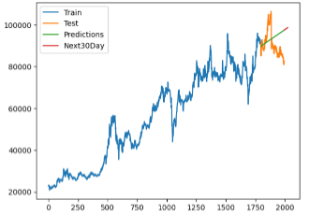
\includegraphics[width=\linewidth]{bibliography/LN_VCB91.png}
    \caption{Linear Regression model's result with 9:1 splitting proportion}
    \label{fig8}
  \end{minipage}
\end{figure}
\begin{figure}[H]
  \centering
  \begin{minipage}{0.8\linewidth}
    \centering
    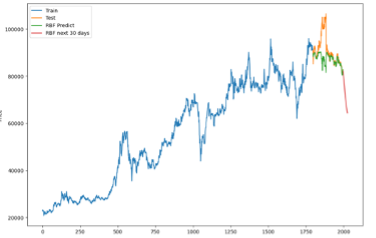
\includegraphics[width=\linewidth]{bibliography/SVR_VCB91.png}
    \caption{ARIMA model's result with 9:1 splitting proportion}
    \label{fig9}
  \end{minipage}
\end{figure}
\begin{figure}[H]
  \centering
  \begin{minipage}{0.8\linewidth}
    \centering
    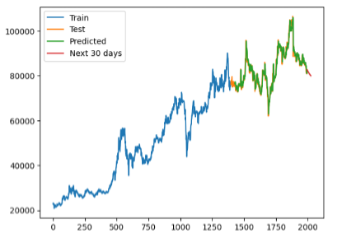
\includegraphics[width=\linewidth]{bibliography/GRU_VCB73.png}
    \caption{VARMA model's result with 7:3 splitting proportion}
    \label{fig10}
  \end{minipage}
\end{figure}
\begin{figure}[H]
  \centering
  \begin{minipage}{0.8\linewidth}
    \centering
    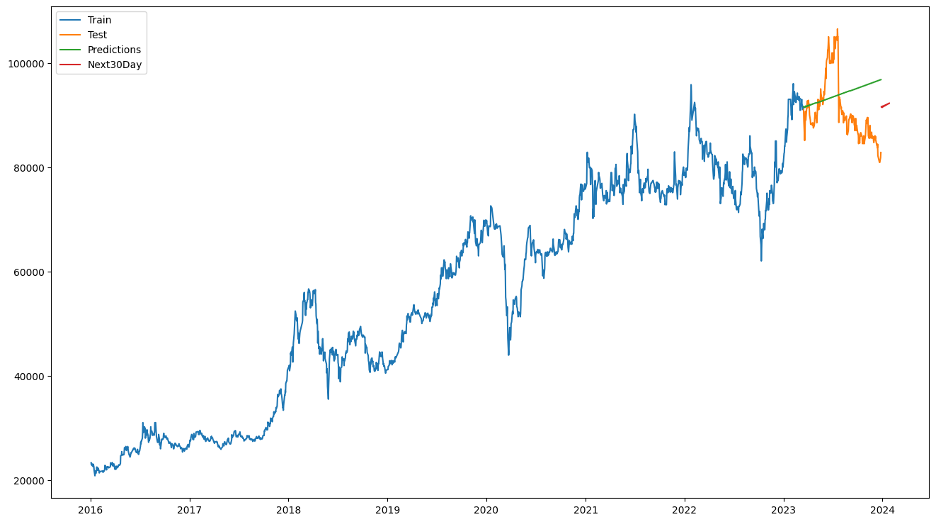
\includegraphics[width=\linewidth]{bibliography/ARIMA_VCB91.png}
    \caption{BaggingRNN model's result with 9:1 splitting proportion}
    \label{fig11}
  \end{minipage}
\end{figure}
\begin{figure}[H]
  \centering
  \begin{minipage}{0.8\linewidth}
    \centering
    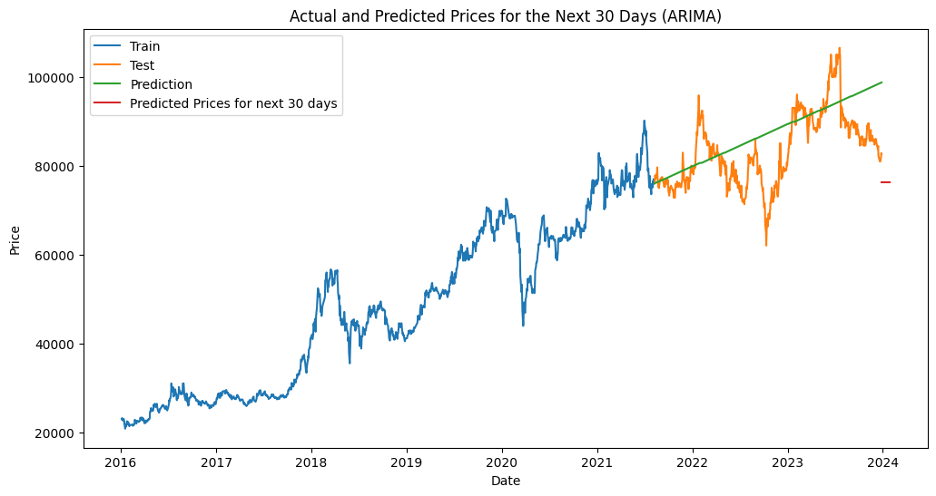
\includegraphics[width=\linewidth]{bibliography/SARIMA_VCB73.png}
    \caption{RNN model's result with 7:3 splitting proportion}
    \label{fig12}
  \end{minipage}
\end{figure}
\begin{figure}[H]
  \centering
  \begin{minipage}{0.8\linewidth}
    \centering
    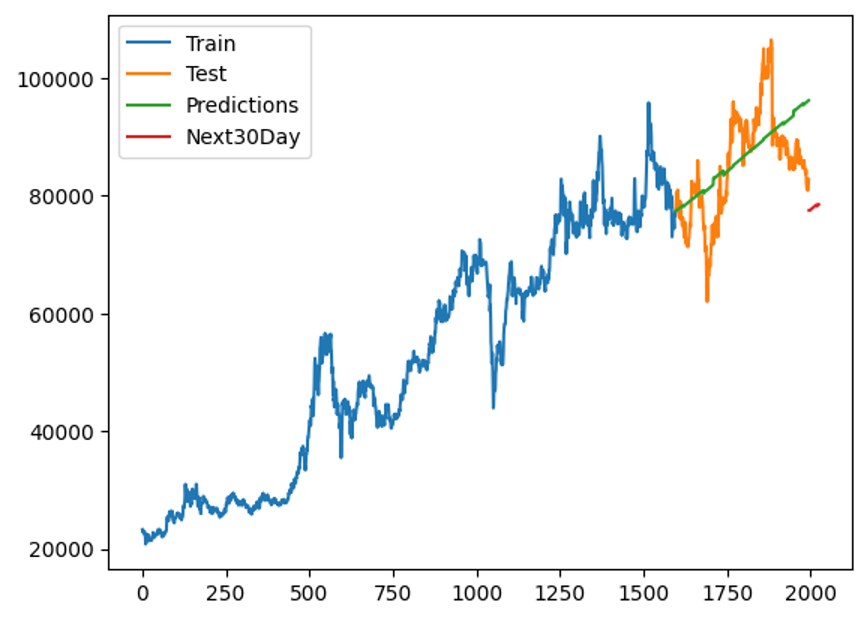
\includegraphics[width=\linewidth]{bibliography/DLM_VCB82.png}
    \caption{GRU model's result with 8:2 splitting proportion}
    \label{fig13}
  \end{minipage}
\end{figure}
\begin{figure}[H]
  \centering
  \begin{minipage}{0.8\linewidth}
    \centering
    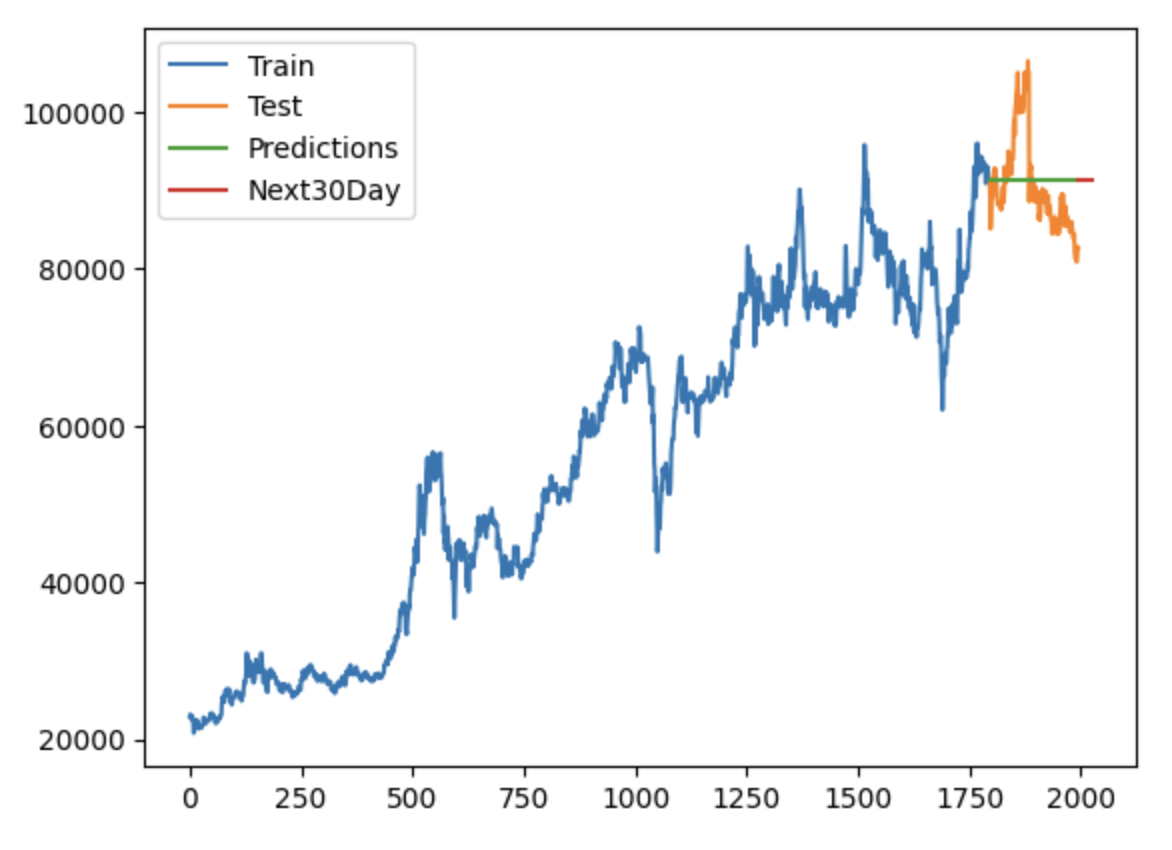
\includegraphics[width=\linewidth]{bibliography/ETS_VCB91.png}
    \caption{LSTM model's result with 9:1 splitting proportion}
    \label{fig14}
  \end{minipage}
\end{figure}
\begin{figure}[H]
  \centering
  \begin{minipage}{0.8\linewidth}
    \centering
    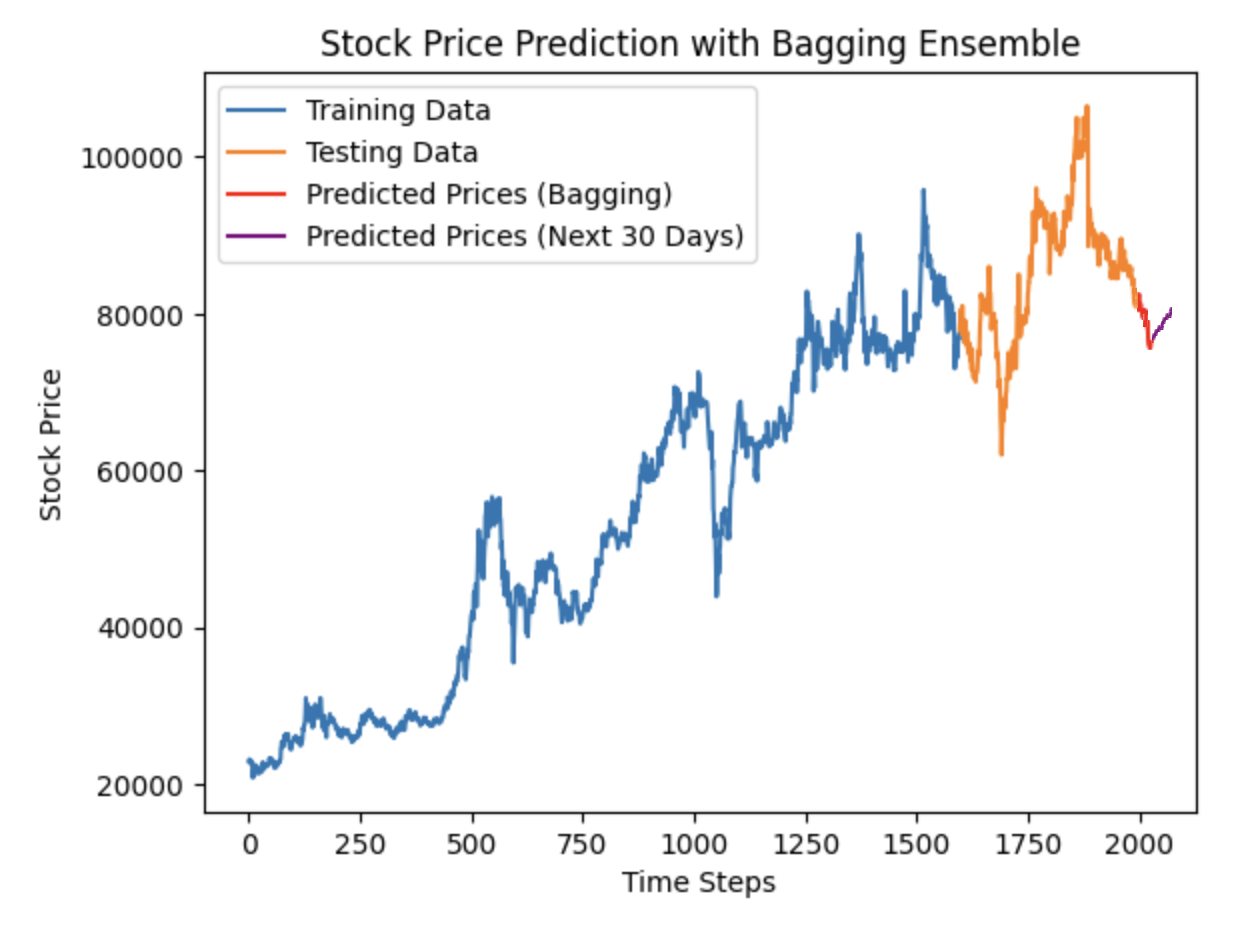
\includegraphics[width=\linewidth]{bibliography/baggingGRU_vcb.png}
    \caption{ResNet model's result with 8:2 splitting proportion}
    \label{bagginggru}
  \end{minipage}
\end{figure}
\subsection{HSG dataset} 
\begin{table}[H]
    \centering
    \begin{tabular}{|c|c|c|c|c|}
         \hline
         \multicolumn{5}{|c|}{\textbf{HSG Dataset's Evaluation}}\\
         \hline
         \centering Model & Training:Testing & RMSE & MAPE (\%) & MAE\\
         \hline
         \multirow{2}{*}{LN} & 7:3 & 20090.74 & 347.93 & 19977.79 \\ & 8:2 & 11622.90 & 212.60 & 11608.38 \\ & \textbf{9:1} & \textbf{6134.12} & \textbf{110.75} & \textbf{6084.42}\\
         \hline
         \multirow{2}{*}{ARIMA} & 7:3&11864.3&7.52&0.021\\ & 8:2&8521.33&5.01&0.009 \\ & \textbf{9:1} & \textbf{7006.54} & \textbf{3.73} & \textbf{0.006}\\
         \hline
         \multirow{2}{*}{VARMA} & 7:3	& 6131.72 & 0.28 & 5345.89 \\ & 8:2 & 5135.90 & 0.06 & 4539.10 \\ & \textbf{9:1} & \textbf{1534.00}  & \textbf{0.06} & \textbf{1316.51}\\
         \hline
         \multirow{2}{*}{BaggingRNN} & 7:3 &  8620.284 &  8.559 & 0.01 \\ & 8:2 &  11729.2 & 10.825 & 0.019 \\ & \textbf{9:1} & \textbf{7644.773}  & \textbf{7.287} & \textbf{0.007}\\
         \hline
         \multirow{2}{*}{RNN} & \textbf{7:3}	& \textbf{7971.644} & \textbf{7.755} & \textbf{0.009} \\ & 8:2 & 11711.484 & 10.809 & 0.019 \\ & 9:1 & 8629.708 & 8.253 & 0.009\\
         \hline
         \multirow{2}{*}{GRU} & 7:3 & 13156.831&13.336 & 0.021 \\ & \textbf{8:2} &	\textbf{7209.84} & \textbf{7.093} & \textbf{0.007} \\ & 9:1 &11945.338	&11.444&0.016\\
         \hline
         \multirow{2}{*}{LSTM} & 7:3 & 10949.0750 & 9.4738 & 0.0169 \\ & 8:2 & 11717.8586 &10.8142 & 0.0189 \\ & \textbf{9:1} &  	\textbf{6000.7953} &	\textbf{5.2412} & 	\textbf{0.004} \\
         \hline
         \multirow{2}{*}{ResNet} & 7:3 & 941.7588 &  1.7384 &  0.0005 \\ & 8:2 & 939.7588 &  1.6546 &  0.0005 \\ & \textbf{9:1} & \textbf{936.8374} & \textbf{1.6273} & \textbf{0.0005}\\
         \hline
    \end{tabular}
    \caption{HSG Dataset's Evaluation}
    \label{mbbresult}
\end{table}

\begin{figure}[H]
  \centering
  \begin{minipage}{0.8\linewidth}
    \centering
    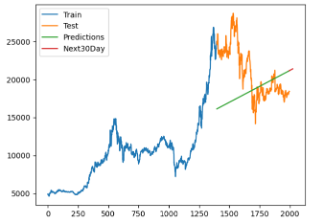
\includegraphics[width=\linewidth]{bibliography/LN_MBB73.png}
    \caption{Linear Regression model's result with 7:3 splitting proportion}
    \label{fig15}
  \end{minipage}
\end{figure}
\begin{figure}[H]
  \centering
  \begin{minipage}{0.8\linewidth}
    \centering
    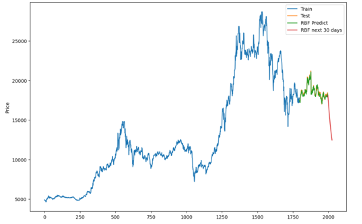
\includegraphics[width=\linewidth]{bibliography/SVR_MBB91.png}
    \caption{ARIMA model's result with 9:1 splitting proportion}
    \label{fig16}
  \end{minipage}
\end{figure}
\begin{figure}[H]
  \centering
  \begin{minipage}{0.8\linewidth}
    \centering
    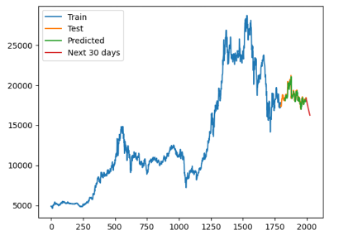
\includegraphics[width=\linewidth]{bibliography/GRU_MBB91.png}
    \caption{VARMA model's result with 9:1 splitting proportion}
    \label{fig17}
  \end{minipage}
\end{figure}
\begin{figure}[H]
  \centering
  \begin{minipage}{0.8\linewidth}
    \centering
    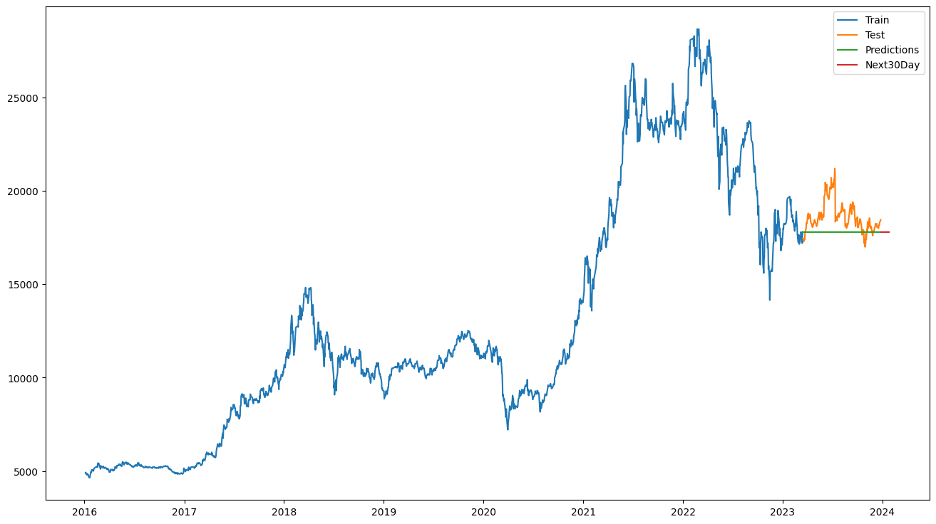
\includegraphics[width=\linewidth]{bibliography/ARIMA_MBB91.png}
    \caption{BaggingRNN model's result with 9:1 splitting proportion}
    \label{fig18}
  \end{minipage}
\end{figure}
\begin{figure}[H]
  \centering
  \begin{minipage}{0.8\linewidth}
    \centering
    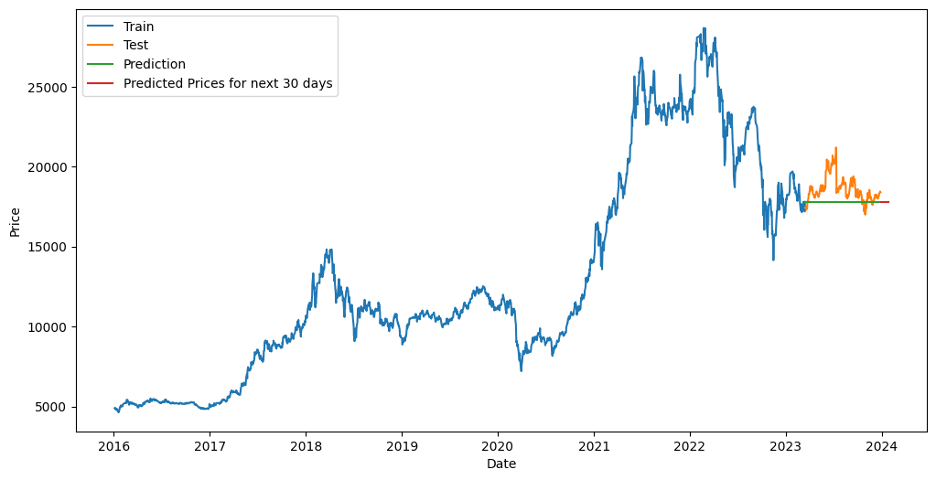
\includegraphics[width=\linewidth]{bibliography/SARIMA_MBB91.png}
    \caption{RNN model's result with 9:1 splitting proportion}
    \label{fig19}
  \end{minipage}
\end{figure}
\begin{figure}[H]
  \centering
  \begin{minipage}{0.8\linewidth}
    \centering
    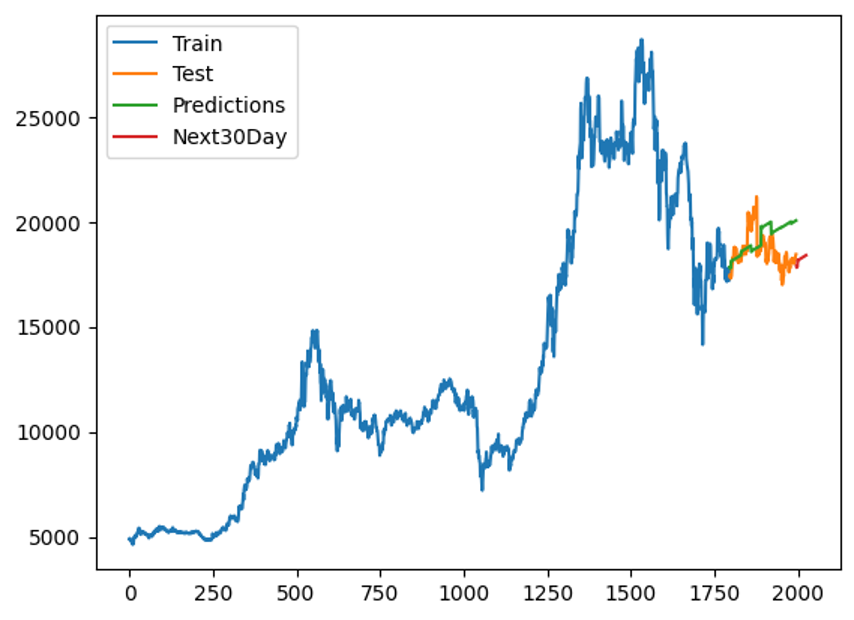
\includegraphics[width=\linewidth]{bibliography/DLM_MBB91.png}
    \caption{GRU model's result with 9:1 splitting proportion}
    \label{fig20}
  \end{minipage}
\end{figure}
\begin{figure}[H]
  \centering
  \begin{minipage}{0.8\linewidth}
    \centering
    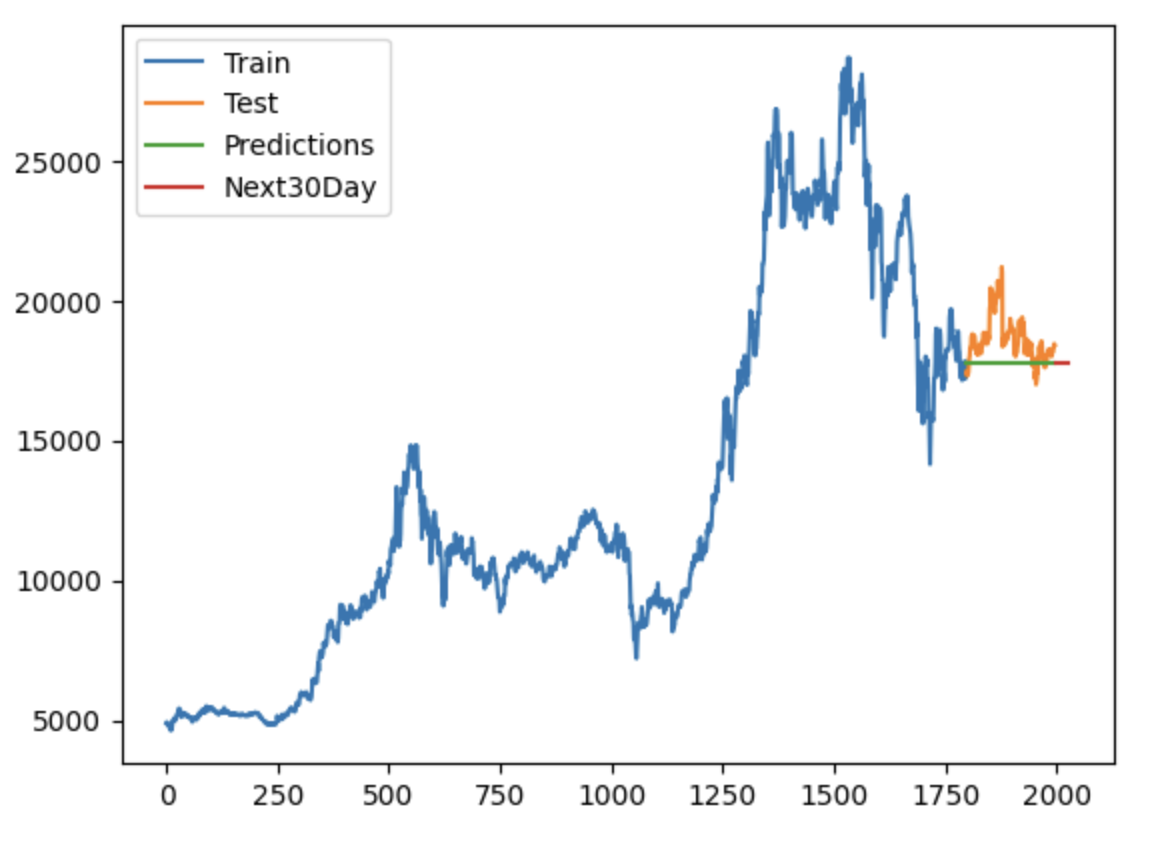
\includegraphics[width=\linewidth]{bibliography/ETS_MBB91.png}
    \caption{LSTM model's result with 9:1 splitting proportion}
    \label{fig21}
  \end{minipage}
\end{figure}
\begin{figure}[H]
  \centering
  \begin{minipage}{0.8\linewidth}
    \centering
    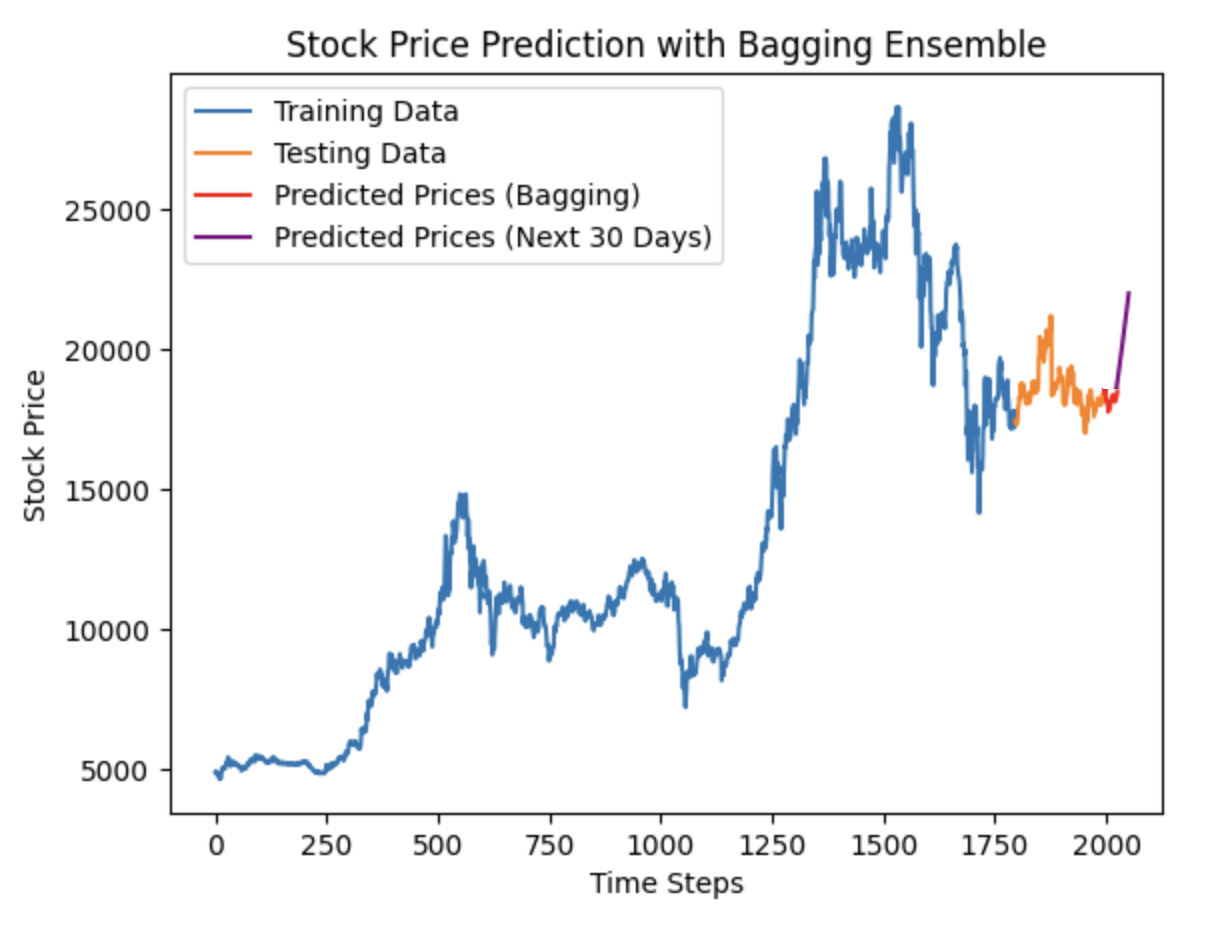
\includegraphics[width=\linewidth]{bibliography/baggingGRU_MBB.png}
    \caption{ResNet model's result with 9:1 splitting proportion}
    \label{mbbbggg}
  \end{minipage}
\end{figure}
\subsection{NKG dataset} 
\begin{table}[H]
    \centering
    \begin{tabular}{|c|c|c|c|c|}
         \hline
         \multicolumn{5}{|c|}{\textbf{NKG Dataset's Evaluation}}\\
         \hline
         \centering Model & Training:Testing & RMSE & MAPE (\%) & MAE\\
         \hline
         \multirow{2}{*}{LN} & 7:3 & 14261.51 & 327.09 & 14247.65 \\ & 8:2 & 6321.35 & 144.61 & 6247.94 \\ & \textbf{9:1} & \textbf{2643.43} & \textbf{59.49} & \textbf{2484.39}\\
         \hline
         \multirow{2}{*}{ARIMA} & 7:3&11864.3&7.52&0.021\\ & 8:2&8521.33&5.01&0.009 \\ & \textbf{9:1} & \textbf{7006.54} & \textbf{3.73} & \textbf{0.006}\\
         \hline
         \multirow{2}{*}{VARMA} & 7:3	& 6645.97 &  0.27 & 5457.52 \\ & 8:2 & 7100.67 & 0.28 & 6290.94 \\ & \textbf{9:1} & \textbf{3565.43}  & \textbf{0.14} & \textbf{3331.86}\\
         \hline
         \multirow{2}{*}{BaggingRNN} & 7:3 &  8620.284 &  8.559 & 0.01 \\ & 8:2 &  11729.2 & 10.825 & 0.019 \\ & \textbf{9:1} & \textbf{7644.773}  & \textbf{7.287} & \textbf{0.007}\\
         \hline
         \multirow{2}{*}{RNN} & \textbf{7:3}	& \textbf{7971.644} & \textbf{7.755} & \textbf{0.009} \\ & 8:2 & 11711.484 & 10.809 & 0.019 \\ & 9:1 & 8629.708 & 8.253 & 0.009\\
         \hline
         \multirow{2}{*}{GRU} & 7:3 & 13156.831&13.336 & 0.021 \\ & \textbf{8:2} &	\textbf{7209.84} & \textbf{7.093} & \textbf{0.007} \\ & 9:1 &11945.338	&11.444&0.016\\
         \hline
         \multirow{2}{*}{LSTM} & 7:3 & 10949.0750 & 9.4738 & 0.0169 \\ & 8:2 & 11717.8586 &10.8142 & 0.0189 \\ & \textbf{9:1} &  	\textbf{6000.7953} &	\textbf{5.2412} & 	\textbf{0.004} \\
         \hline
         \multirow{2}{*}{ResNet} & 7:3 & 941.7588 &  1.7384 &  0.0005 \\ & 8:2 & 939.7588 &  1.6546 &  0.0005 \\ & \textbf{9:1} & \textbf{936.8374} & \textbf{1.6273} & \textbf{0.0005}\\
         \hline
    \end{tabular}
    \caption{NKG Dataset's Evaluation}
    \label{mbbresult}
\end{table}

\begin{figure}[H]
  \centering
  \begin{minipage}{0.8\linewidth}
    \centering
    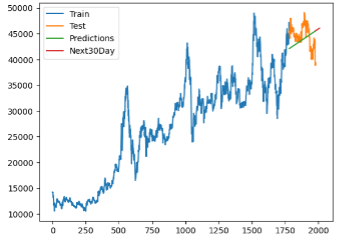
\includegraphics[width=\linewidth]{bibliography/LN_BIDV91.png}
    \caption{Linear Regression model's result with 9:1 splitting proportion}
    \label{fig22}
  \end{minipage}
\end{figure}
\begin{figure}[H]
  \centering
  \begin{minipage}{0.8\linewidth}
    \centering
    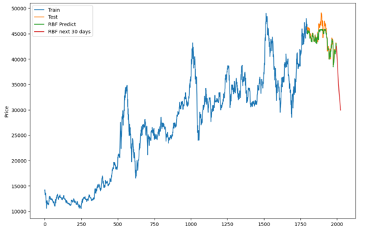
\includegraphics[width=\linewidth]{bibliography/SVR_BIDV91.png}
    \caption{ARIMA model's result with 9:1 splitting proportion}
    \label{fig23}
  \end{minipage}
\end{figure}
\begin{figure}[H]
  \centering
  \begin{minipage}{0.8\linewidth}
    \centering
    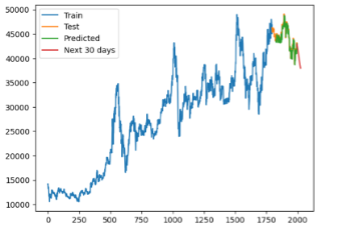
\includegraphics[width=\linewidth]{bibliography/GRU_BIDV91.png}
    \caption{VARMA model's result with 9:1 splitting proportion}
    \label{fig24}
  \end{minipage}
\end{figure}
\begin{figure}[H]
  \centering
  \begin{minipage}{0.8\linewidth}
    \centering
    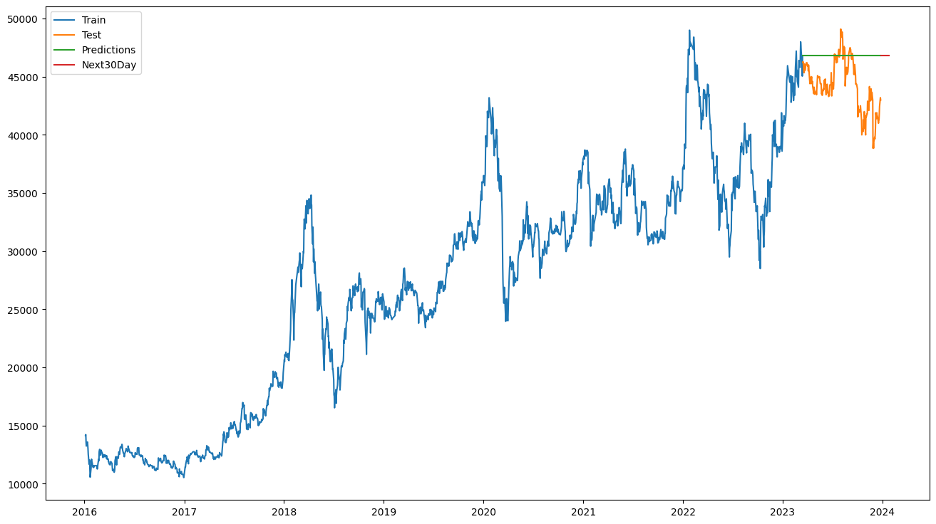
\includegraphics[width=\linewidth]{bibliography/ARIMA_BIDV91.png}
    \caption{BaggingRNN model's result with 9:1 splitting proportion}
    \label{fig25}
  \end{minipage}
\end{figure}
\begin{figure}[H]
  \centering
  \begin{minipage}{0.8\linewidth}
    \centering
    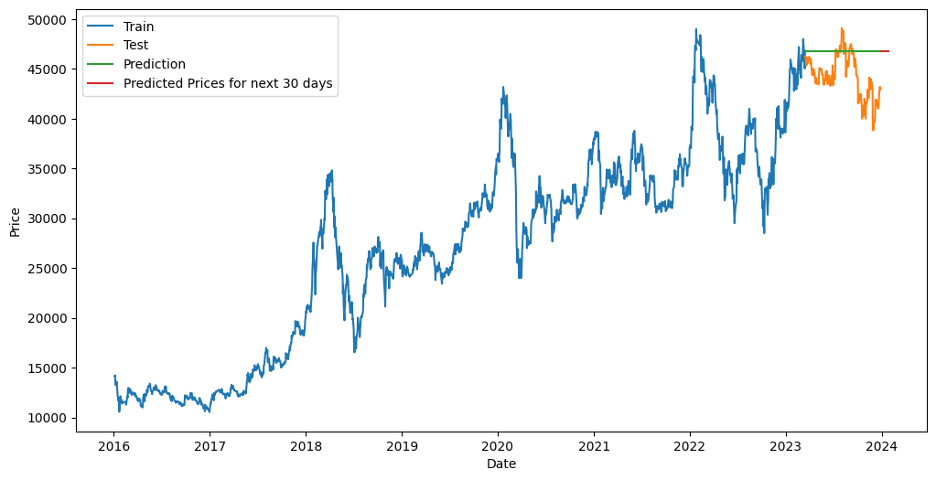
\includegraphics[width=\linewidth]{bibliography/SARIMA_BIDV91.png}
    \caption{RNN model's result with 9:1 splitting proportion}
    \label{fig26}
  \end{minipage}
\end{figure}
\begin{figure}[H]
  \centering
  \begin{minipage}{0.8\linewidth}
    \centering
        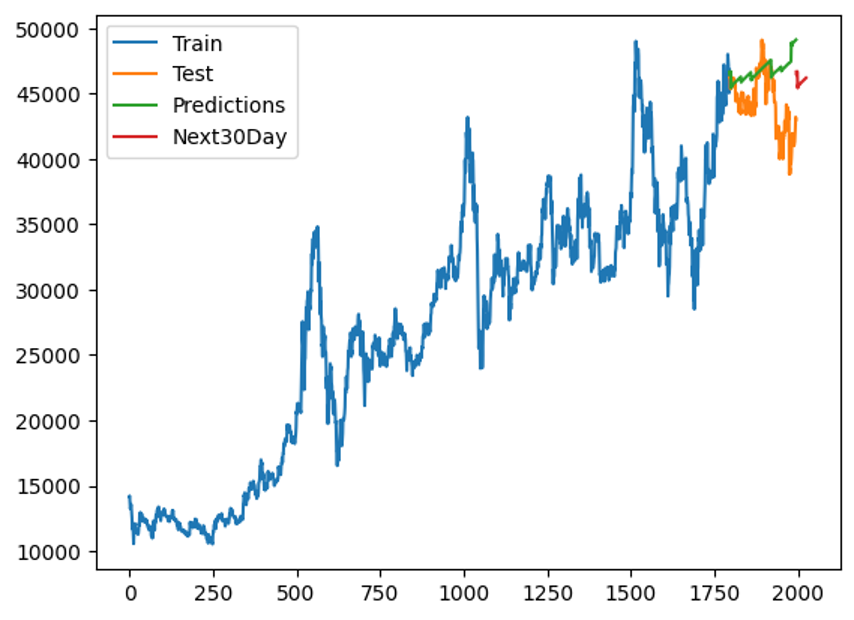
\includegraphics[width=\linewidth]{bibliography/BIDV_DLM91.png}
    \caption{GRU model's result with 9:1 splitting proportion}
    \label{fig27}
  \end{minipage}
\end{figure}
\begin{figure}[H]
  \centering
  \begin{minipage}{0.8\linewidth}
    \centering
        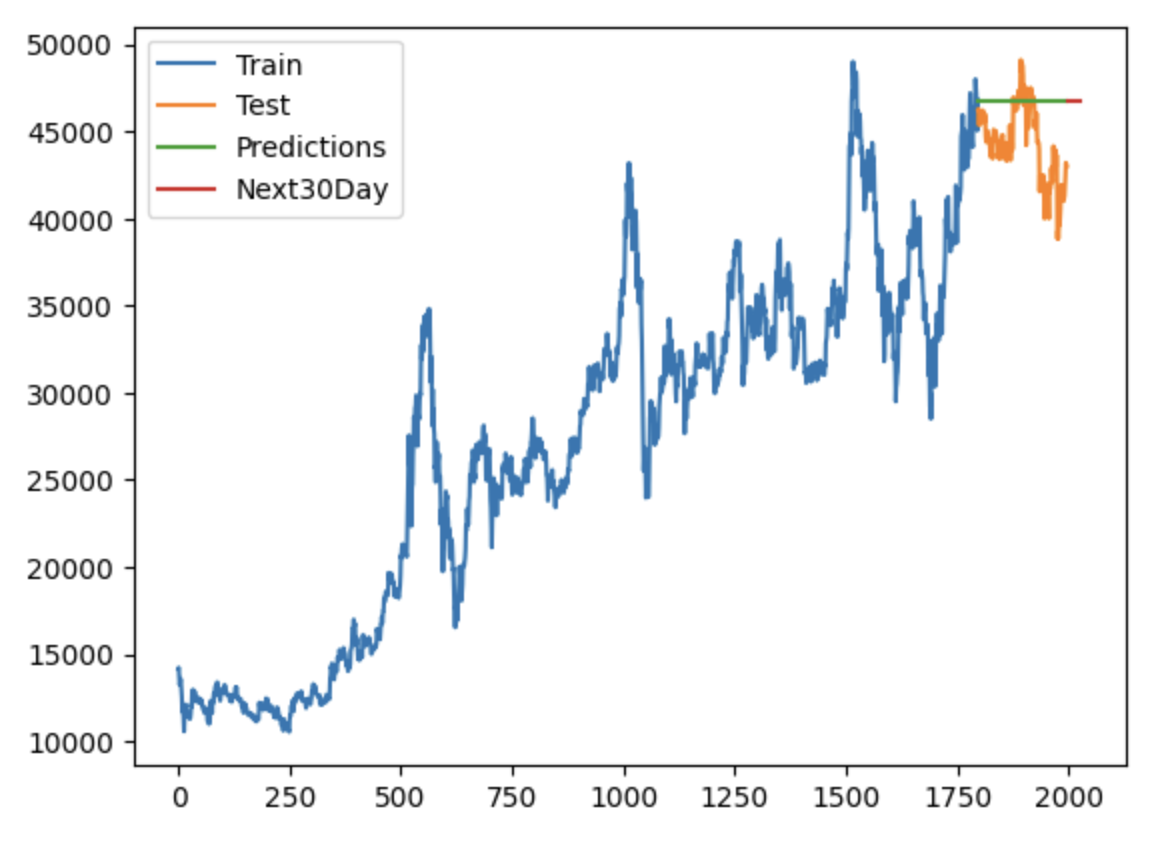
\includegraphics[width=\linewidth]{bibliography/ETS_BIDV91.png}
    \caption{LSTM model's result with 9:1 splitting proportion}
    \label{fig28}
  \end{minipage}
\end{figure}
\begin{figure}[H]
  \centering
  \begin{minipage}{0.8\linewidth}
    \centering
        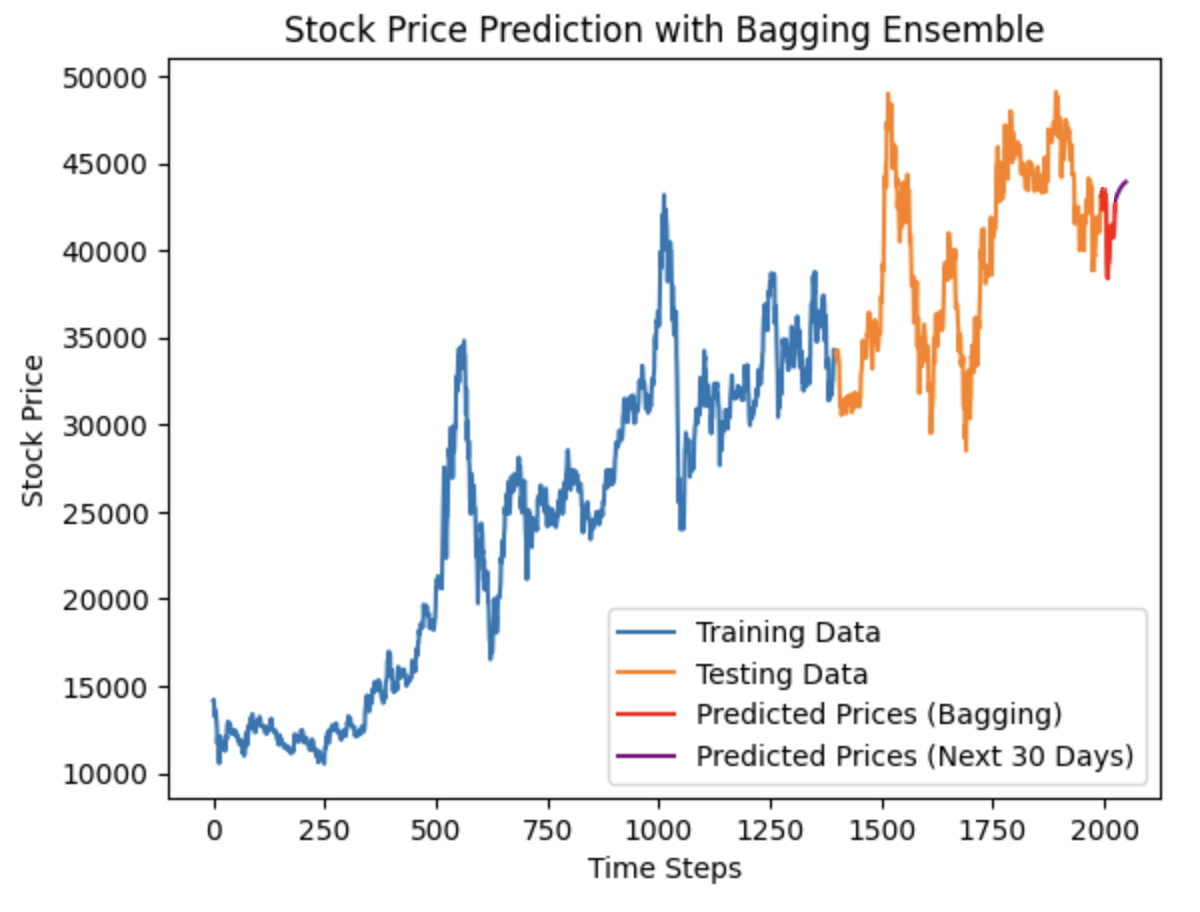
\includegraphics[width=\linewidth]{bibliography/baggingGRU_BIDV.png}
    \caption{ResNet model's result with 7:3 splitting proportion}
    \label{fig28}
  \end{minipage}
\end{figure}
\section{Conclusion}
\subsection{Summary}
%In the achievement of forecasting stock prices, the exploration of diverse methodologies, ranging from traditional statistical models to advanced machine learning algorithms, has been aimed. Among the performed models, Linear Regression (LR), Auto Regressive Integrated Moving Average (ARIMA), Support Vector Regression (SVR), Seasonal Auto Regression Integrated Moving Average (SARIMA), Dynamic Linear Model (DLM), Bagging – GRU, and Simple Exponential Smoothing (SES), it becomes evident that Support Vector Regression (SVR), Gated Recurrent Unit (GRU), and Bagging GRU emerge as the most promising and effective models for predicting stock prices.\\
%The intricacies of stock price forecasting, rooted in the complexity and unpredictability of financial markets, demand models that can capture nuanced patterns and relationships within the data. Support Vector Regression (SVR) showcases its efficacy in handling intricate relationships, providing robust predictions. Gated Recurrent Unit (GRU) models, with their ability to capture sequential dependencies, exhibit notable performance in forecasting stock prices. The introduction of ensemble learning through Bagging GRU further refines the predictive capabilities, offering a collective insight that surpasses individual models.\\
%As evidenced by the evaluation metrics, including RMSE, MAPE, and MSLE, the SVR, GRU, and Bagging GRU models consistently demonstrate superior performance across various aspects of forecasting accuracy. Their adaptability to handle the inherent uncertainties of stock markets positions them as formidable tools for investors and analysts seeking reliable predictions.
\subsection{Future Considerations}
%In our future research, it is crucial to prioritize further optimization of the previously mentioned models. This optimization effort should specifically focus on:\\
%\indent\textbullet\ Enhancing the accuracy of the model. While the above algorithms have demonstrated promising results in predicting stock prices, there is a need to further improve the model's accuracy to ensure more precise forecasting outcomes.\\
%\indent\textbullet\ Exploring alternative machine learning algorithms or ensemble techniques. Ensemble techniques, such as combining multiple models or using various ensemble learning methods, can also improve the robustness and accuracy of the forecasts.\\
%\indent\textbullet\ Researching new forecasting models. The field of forecasting continuously evolves, with new algorithms and models being researched and developed. It is crucial to stay updated with these approaches and explore new forecasting models that offer improved accuracy and performance. \\
%By continuously exploring and incorporating new features, data sources, and modeling techniques, we can strive for ongoing optimization of the forecasting models and enhance their ability to predict stock prices with greater precision and reliability.
\section*{Acknowledgment}
\addcontentsline{toc}{section}{Acknowledgment}
%First and foremost, we would like to express our sincere gratitude to \textbf{Assoc. Prof. Dr. Nguyen Dinh Thuan} and \textbf{Mr. Nguyen Minh Nhut} for their exceptional guidance, expertise, and invaluable feedback throughout the research process. Their mentorship and unwavering support have been instrumental in shaping the direction and quality of this study. Their profound knowledge, critical insights, and attention to detail have significantly contributed to the success of this research.
%\\This research would not have been possible without the support and contributions of our mentors. We would like to extend our heartfelt thanks to everyone involved for their invaluable assistance, encouragement, and belief in our research. Thank you all for your invaluable assistance and encouragement.

%% UNCOMMENT these lines below (and remove the 2 commands above) if you want to embed the bibliografy.
\begin{thebibliography}{00}

\bibitem{b1} Warsono, Edwin Russel, Wamiliana, Widiarti and Mustofa Usman, ''Modeling and Forecasting by the Vector Autoregressive Moving
Average Model for Export of Coal and Oil Data (Case Study from
Indonesia over the Years 2002-2017)'' June 2019. Retrieved from \(doi.org/10.32479/ijeep.7605\)

\bibitem{b2} Punnee Sittidech, Nongyao Nai-arun, and Ian T. Nabney, ''Bagging Model with Cost Sensitive Analysis on Diabetes Data'', January - June 2015. Retrieved from \(publications.aston.ac.uk/id/eprint/27369/1/689_1255_1_SM.pdf\)

\bibitem{b3} Hyungeun Choi, Seunghyoung Ryu and Hongseok Kim, ''Short-Term Load Forecasting based on ResNet and LSTM'', October 2018. Retrieved from \(doi.org/10.1109/SmartGridComm.2018.8587554\)

\bibitem{b4} Gers, F. A., Schmidhuber, J., & Cummins, F. (2000). Learning to forget: Continual prediction with LSTM. Neural computation, 12(10), 2451-2471. \

\bibitem{b5} Graves, A., & Schmidhuber, J. (2005). Framewise phoneme classification with bidirectional LSTM and other neural network architectures. Neural Networks, 18(5-6), 602-610. \
\end{thebibliography}
%%%%%%%%%%%%%%%


\EOD

\end{document}
